%!TEX root = ../../main.tex


\begin{figure}[p]
{\footnotesize\texthv{\textbf{(a) All alleles analysed}}} \\
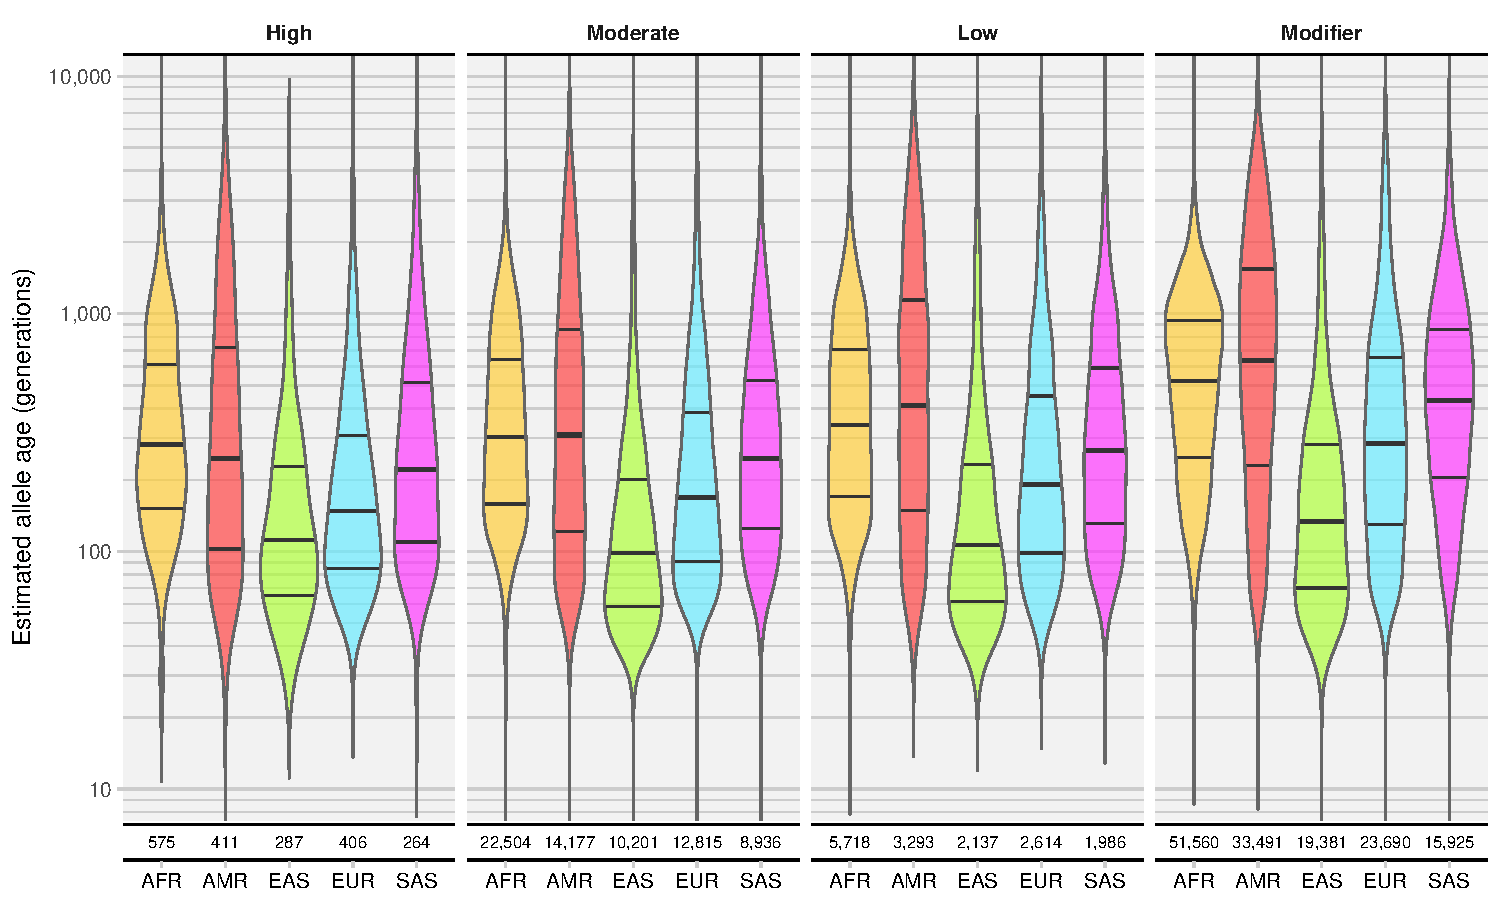
\includegraphics[width=\textwidth]{./img/ch5/1kg_pop_impact_a}
{\footnotesize\texthv{\textbf{(b) Population-specific alleles}}} \\
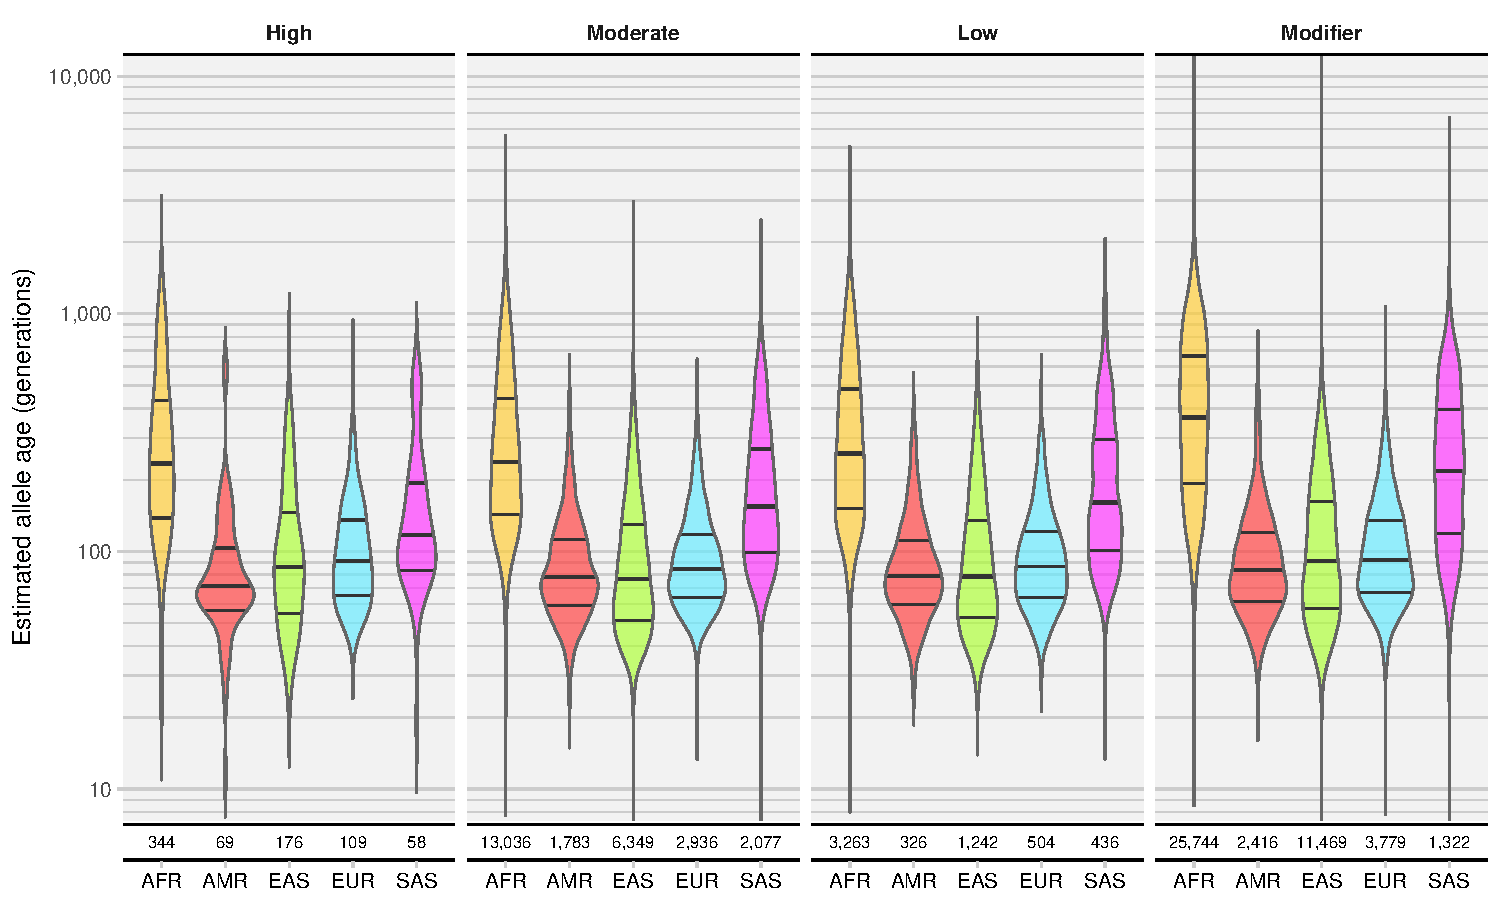
\includegraphics[width=\textwidth]{./img/ch5/1kg_pop_impact_b}
\Caption{Allele age after correction on population-specific frequency in 1000 Genomes}%
{The distribution of inferred allele age is shown in Violin plots by predicted impact category for each population in the \gls{1kg} dataset; \nth{1}, \nth{2}, and \nth{3} quartiles are indicated.
In Panel~\textbf{(a)}, all variants retained after quality control were included in the comparison, which included ${n = \num{141069}}$ target sites.
Note that this also included alleles shared among populations.
In Panel~\textbf{(b)}, only the subset of population-specific variants was included (${n = \num{77438}}$).
The number of alleles retained in each impact category and population are shown below each graph.
The colours used follow the \gls{1kg} colour-scheme.}%
{fig:1kg_pop_impact}
\end{figure}
